\subsection{PHÂN LOẠI, PHƯƠNG PHÁP GIẢI TOÁN}
\begin{dang}{Xác định ảnh của một hình qua phép chiếu song song}
\end{dang}
\begin{vd}
	Cho hình hộp $ABCD.A'B'C'D'$.
	\begin{itemize}
		\item [a)] Xác định ảnh của các điểm $A', B', C', D'$ qua phép chiếu song song lên mặt phẳng $(ABCD)$ theo phương $AA'$.
		\item [b)] Xác định ảnh của tam giác $A'C'D'$ qua phép chiếu song song lên mặt phẳng $(ABCD)$ theo phương $A'B$.
	\end{itemize}
	\loigiai{
		\begin{itemize}
			\item 	Vì các cạnh $AA',BB', CC', DD'$ song song nhau nên $A, B, C, D$ là hình chiếu của $A', B', C', D'$.
			\item 
		\end{itemize}
	
	}
\end{vd}
\begin{vd}
	Phép chiếu song song biến hình bình hành $ABCD$ thành hình bình hành $A'B'C'D'$. Chứng minh rằng phép chiếu đó biến tâm của hình bình hành $ABCD$ thành tâm của hình bình hành $A'B'C'D'$.
	\loigiai{
		Gọi $O$ là tâm hình bình hành $ABCD$, suy ra $O$ là trung điểm của $AC$.
		\\Phép chiếu song song biến $O$ thành $O'$.\\
		Ta có $A, O, C $ thẳng hàng theo thứ tự đó và $\dfrac{OA}{OC}=1$ nên ba điểm $A', O', C'$ thẳng hàng theo thứ tự đó và $\dfrac{O'A'}{O'C'}=1$. Suy ra $O'$ là trung điểm của $A'C'$.\\
		Vậy $O'$ là tâm của hình bình hành $A'B'C'D'$.
	}
\end{vd}
\begin{vd}
	Phép chiếu song song biến tam giác $ABC$  thành tam giác $A'B'C'$ . Chứng minh rằng phép chiếu đó biến đường trung bình của tam giác $ABC$  thành đường trung bình của tam giác $A'B'C'$  .
	\loigiai{
	Gọi $M ,N$   lần lượt là trung điểm $AB ,AC$   nên  $MN$ là đường trung bình của tam giác $ABC$.\\
	Phép chiếu song song biến $M$  thành $M'$ , biến $N$  thành $N'$ .\\
	Ta có ba điểm  $A, M , B$  thẳng hàng theo thứ tự đó và $\dfrac{AM}{AB}=\dfrac{1}{2}$  nên ba điểm $A' ,M'  , B'$  thằng hàng theo thứ tự đó và $\dfrac{A'M'}{A'B'}=\dfrac{1}{2}$ . Suy ra $M'$   là trung điểm $A'B'$ .\\
	Tương tự $N'$  là trung điểm $A'C'$ .\\
	Vậy $M'N'$  là đường trung bình của tam giác $A'B'C'$ .
	
}
\end{vd}
\begin{dang}{Vẽ hình biểu diễn của một số hình khối đơn giản}
\end{dang}
\begin{vd}
	Vẽ hình biểu diễn của các hình sau
\begin{itemize}
	\item [a)] Hình lục giác đều.
	\item [b)] Hình vuông nội tiếp trong hình tròn.
\end{itemize}
\end{vd}
\begin{vd}
	Vẽ hình biểu diễn của hình chóp $S.ABCD$ có đáy là hình thang $ABCD$ với $AB$ song song $CD$; $AB=2$ cm, $CD=6$ cm.
	\loigiai{
	\immini{Vì hình chóp $S.ABCD$ có $AB \parallel CD$ và $AB=2$ cm, $CD=6$ cm nên hình biễu diễn của hình chóp cũng có đáy $AB \parallel CD$ và $\dfrac{AB}{CD}=\dfrac{2}{6}=\dfrac{1}{3}$.\\
	Do đó, ta vẽ hình thang $ABCD$ có $AB \parallel CD$ và $AB=\dfrac{1}{3} CD$, vẽ điểm $S$ và nối $SA$, $SB$, $SC$, $SD$.}{
	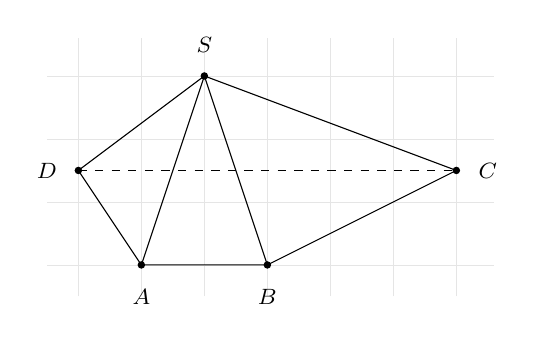
\begin{tikzpicture}[scale=0.8, font=\footnotesize,>=stealth]
		\path
		%	Vẽ mp
		(0,0) coordinate (A)
		(2,0) coordinate (B)
		(5,1.5) coordinate (C)
		(-1,1.5) coordinate (D)
		(1,3) coordinate (S)
		;
		\draw[line width=0.1pt,gray!20!white] (-1.5,-0.5) grid (5.6,3.6);
		\draw (A)--(B)--(C)--(S)--(D)--(A)--(S) (C)--(S)--(B);
		\draw[dashed] (D)--(C);
		\foreach \x/\g in {A/-90,B/-90,C/0,D/180,S/90}\draw[fill=black] (\x) circle (.05) +(\g:.5)node{\footnotesize$\x$};
	\end{tikzpicture}
}
}

\end{vd}
\begin{vd}
	Vẽ hình biểu diễn của các hình sau
	\begin{itemize}
		\item [a)] Hình lăng trụ có đáy là tam giác đều.
		\item [b)] Hình lăng trụ có đáy là lục giác đều.
		\item [c)] Hình hộp.
		\item [d)] Hình chóp tam giác $S.ABC$ đặt trên một hình lăng trụ tam giác $ABC.A'B'C'$.
	\end{itemize}
\end{vd}
